\documentclass{standalone}
\usepackage{amsmath}
\usepackage{amssymb}
\usepackage{fontspec}
  \setmainfont{Latin Modern Roman}
\usepackage{unicode-math}
  \setmathfont{Latin Modern Math}[FakeBold=1.2]
\usepackage{tikz}
  \usetikzlibrary{positioning, arrows.meta, calc}

% Document metadata
\title{Chapter 03 — section 04 — diagram 26}
\author{0im}
\date{2277}

\begin{document}
  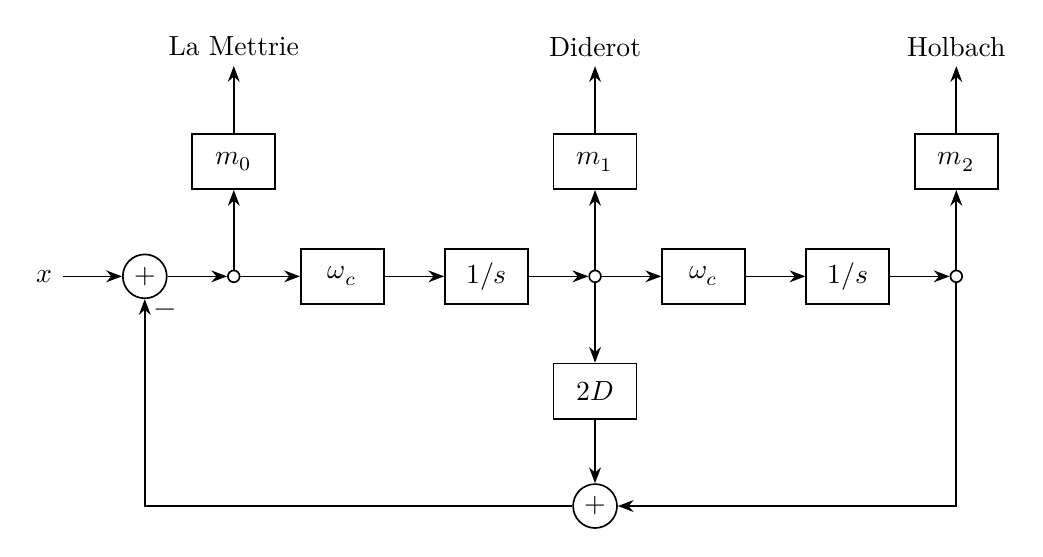
\begin{tikzpicture}
  [
    on grid,
    node distance=4.15em and 2.15em, % Fixed: Added explicit em units
    block/.style={draw, rectangle, minimum height=2em, minimum width=3em, semithick},
    sum/.style={draw, circle, inner sep=2pt, semithick},
    branch/.style={draw, circle, inner sep=1.5pt, semithick}
  ]
    % =========================================================================
    % NODES
    % =========================================================================
    \node (x) at (0,0) {$x$};
    \node [sum, right=of x.east, anchor=west] (sum1) {$+$};
    \node [branch, right=of sum1.east, anchor=west] (branch1) {};
    \node [block, right=of branch1.east, anchor=west] (cutoff1) {$\omega_c$};
    \node [block, right=of cutoff1.east, anchor=west] (integrator1) {$1/s$};
    \node [branch, right=of integrator1.east, anchor=west] (branch2) {};
    \node [block, right=of branch2.east, anchor=west] (cutoff2) {$\omega_c$};
    \node [block, right=of cutoff2.east, anchor=west] (integrator2) {$1/s$};
    \node [branch, right=of integrator2.east, anchor=west] (branch3) {};

    \node [block, above=of branch1] (m0) {$m_0$};
    \node [above=of m0] (y1) {La Mettrie};

    \node [block, above=of branch2] (m1) {$m_1$};
    \node [above=of m1] (y2) {Diderot};

    \node [block, above=of branch3] (m2) {$m_2$};
    \node [above=of m2] (y3) {Holbach};

    \node [block, below=of branch2] (k) {$2D$};
    \node [sum, below=of k] (sum2) {$+$};

    \node [below=of sum1] (blank1) {};
    \node [below=of branch3] (blank2) {};
    \node [below=of blank1] (blank3) {};
    \node [below=of blank2] (blank4) {};

    % =========================================================================
    % PATHS
    % =========================================================================
    % --- HORIZONTAL ---
    \draw [-Stealth, semithick] (x.east) -- (sum1.west);
    \draw [-Stealth, semithick] (sum1.east) -- (branch1.west);
    \draw [-Stealth, semithick] (branch1.east) -- (cutoff1.west);
    \draw [-Stealth, semithick] (cutoff1.east) -- (integrator1.west);
    \draw [-Stealth, semithick] (integrator1.east) -- (branch2.west);
    \draw [-Stealth, semithick] (branch2.east) -- (cutoff2.west);
    \draw [-Stealth, semithick] (cutoff2.east) -- (integrator2.west);
    \draw [-Stealth, semithick] (integrator2.east) -- (branch3.west);
    % --- VERTICAL ---
    \draw [-Stealth, semithick] (branch1.north) -- (m0.south);
    \draw [-Stealth, semithick] (m0.north) -- (y1.south);
    \draw [-Stealth, semithick] (branch2.north) -- (m1.south);
    \draw [-Stealth, semithick] (m1.north) -- (y2.south);
    \draw [-Stealth, semithick] (branch3.north) -- (m2.south);
    \draw [-Stealth, semithick] (m2.north) -- (y3.south);
    \draw [-Stealth, semithick] (branch2.south) -- (k.north);
    \draw [-Stealth, semithick] (k.south) -- (sum2.north);
    % --- ANGLED ---
    \draw [-Stealth, semithick] (sum2.west) -- (blank3.center) -- (sum1.south)
      node [anchor=north west] {$-$};
    \draw [-Stealth, semithick] (branch3.south) -- (blank4.center) -- (sum2.east);

  \end{tikzpicture}

\end{document}